\documentclass[a4paper]{report}

\usepackage[utf8]{inputenc}
\usepackage[english]{babel}
\usepackage[T1]{fontenc}

\usepackage{geometry}
\usepackage{amssymb}
\usepackage{amsmath}
\usepackage{ifthen}
\usepackage{caption}
\usepackage{graphicx}
\usepackage{subcaption}
\usepackage{minted}
\usepackage{siunitx}
\usepackage[version=4]{mhchem}
\usepackage[dvipsnames]{xcolor}
\usepackage[ED=MEGEP-DyF, Ets=ISAE]{tlsflyleaf/tlsflyleaf}
\usepackage{array}
\usepackage{tcolorbox}


\renewcommand*{\vec}[1]{\underline{#1}}
\newcommand*{\mat}[1]{\vec{\vec{#1}}}
\newcommand{\norm}[2][]{\left\|{#2}\right\|\ifthenelse{\equal{#1}{}}{}{_{{#1}}}}
\newcommand{\RKBar}{\rule[-1.1ex]{0pt}{0pt} \\ \hline \rule{0pt}{2.6ex} &}
\newcommand{\transpose}[1]{{#1}^T}
\newcommand{\krylov}[2][]{\ifthenelse{\equal{#1}{}}{\mathcal{K}_{#2}}{\mathcal{K}_{#2}\left({#1}\right)}}

\newcolumntype{M}[1]{>{\centering\arraybackslash}m{#1}}

\usepackage[pdfpagelabels]{hyperref}
% \hypersetup{
%     colorlinks,
%     linkcolor=black,
%     citecolor=black,
%     % filecolor=black,
%     % urlcolor=black
% }

\newcommand{\GP}[1]{\textbf{\color{BurntOrange}{#1}}}
\newcommand{\LM}[1]{\textbf{\color{ForestGreen}{#1}}}
\newcommand{\PS}[1]{\textbf{\color{Red}{#1}}}
\renewcommand{\GP}[1]{}
\renewcommand{\LM}[1]{}
\renewcommand{\PS}[1]{}


\title{\textbf{\large Méthodologies permettant l'obtention efficace de solutions multi-physiques stationnaires pour des applications en énergétique}}
\author{Pierre Seize}
\defencedate{TBD}
\lab{Office National d'Études et de Recherches Aérospatiales - Département Multi-Physique pour l'Énergétique}
% \\ OU \\ ISAE-ONERA EDyF Energétique et Dynamique des Fluides}
\njudge{7}
\nboss{2}
\nreferee{2}
\makesomeone{judge}{1}{Jocelyne ERHEL}{Directrice de recherche}{Membre du jury}
\makesomeone{judge}{2}{Pierre-Henri MAIRE}{Directeur de recherche}{Membre du jury}
\makesomeone{judge}{3}{Xavier VASSEUR}{Docteur, HDR}{Membre du jury}
\makesomeone{judge}{4}{Rodolphe TURPAULT}{Professeur des Universités}{Rapporteur}
\makesomeone{judge}{5}{Vincent PERRIER}{Chargé de recherche, HDR}{Rapporteur}
\makesomeone{judge}{6}{Guillaume PUIGT}{Directeur de recherche}{Directeur de thèse}
\makesomeone{judge}{7}{Lionel MATUSZEWSKI}{Docteur}{Co-Directeur de thèse}
\makesomeone{referee}{1}{Rodolphe TURPAULT}{Professeur des Universités}{}
\makesomeone{referee}{2}{Vincent PERRIER}{Chargé de recherche}{}
\makesomeone{boss}{1}{Guillaume PUIGT}{}{}
\makesomeone{boss}{2}{Lionel MATUSZEWSKI}{}{}


\begin{document}

\pagenumbering{Alph}
\maketitle
\pagenumbering{arabic}

\tableofcontents
\addcontentsline{toc}{chapter}{Table of contents}


\chapter*{Introduction}
\addcontentsline{toc}{chapter}{Introduction}


  \section*{Contexte}

    \paragraph{}
    Ce travail s'ancre dans le domaine de la simulation numérique de la dynamique des fluides, appliquée à l'énergétique.
    Ce domaine regroupe de nombreux acteurs industriels (Ariane group, DGA, Safran, Airbus, ...) ainsi qu'académiques (ONERA, CERFACS, DLR, universités, ...).
    Il s'intéresse à la manière de simuler avec un calculateur un écoulement fluide en essayant de représenter fidèlement la réalité physique.
    Les différents acteurs de ce domaine ont besoin de pouvoir accéder à certaines grandeurs physiques associées à des phénomènes et à des régimes de fonctionnement bien particuliers.
    Il arrive souvent que ces régimes ne soient pas réalisables à notre échelle, en raison de limitations matérielles ou financières.
    On peut prendre comme exemple l’étude du givrage qui a lieu sur la voilure d’un avion, qui est réalisable expérimentalement mais représente un budget imposant pour l’avionneur, ou bien l’étude des transferts thermiques d’une capsule de rentrée atmosphérique, bien plus difficile à réaliser expérimentalement.
    Pour contourner ces limitations, la simulation numérique est la meilleure option, car elle permet de modéliser un tel cas d’étude par l’exécution d’un programme informatique, et d’obtenir un ensemble important de données qui seront analysées par la suite pour répondre aux questions souhaitées.
    L'analyse de la physique produit en général un ensemble d'équations, souvent des équations aux dérivées partielles, représentant le système réel que l'on souhaite étudier.
    Des algorithmes sont alors nécessaires pour déterminer l'écoulement fluide à partir de ces équations, dans le domaine de travail, en fonction du temps.
    Ainsi, pour obtenir les grandeurs souhaitées, le système physique est intégré temporellement à l'aide d'algorithmes mathématiques afin d'obtenir son évolution dans le temps.
    Souvent, le résultat attendu n'est pas l'évolution temporelle complète du système, mais seulement l'obtention de son état d'équilibre.
    On parle alors de simulation stationnaire, en opposition aux simulations instationnaires, qui cherchent à décrire correctement l'évolution temporelle du système.

    \paragraph{}
    Pour l'ensemble de ces acteurs, l'enjeu le plus crucial est de parvenir à obtenir un bon compromis entre temps de calcul et fidélité du résultat.
    En effet, un calcul rapide à tendance à être peu fidèle à la physique, alors qu'un calcul fidèle tend à utiliser plus de ressources informatiques que celles à disposition.
    Pour un calcul stationnaire, la rapidité correspond au fait d'obtenir la solution \emph{convergée} à un faible coût de calcul et humain.
    Cela ce traduit alors par un compromis entre une simulation très coûteuse en ressources informatiques, prenant un temps long, et qui donne des résultats précis et proches de la physique, et une simulation rapide, économe en ressources, mais pour laquelle les résultats ne sont pas significatifs.
    La nécessité de ce compromis vient du fait des algorithmes utilisés dans ces simulations, ainsi que des paramètres donnés à ces algorithmes.
    Une personne développant un outil de simulation numérique doit donc choisir les algorithmes à utiliser pour obtenir un compromis qu'il estime satisfaisant.
    L'intérêt final pour un acteur dans la simulation numérique de la dynamique des fluides est donc d'avoir un résultat suffisamment précis et suffisamment peu cher à obtenir.
    Un résultat précis est nécessaire pour répondre aux questions qui ont nécessité la simulation.
    La recherche d'un résultat peu cher à obtenir est motivée par des questions d'économies en coût de calcul.
    Ce coût englobe le coût en temps de la simulation, payé par l'utilisateur (et indirectement par l'employeur au travers du salaire) et le coût en ressources informatiques payé par l'employeur, c'est à dire en électricité et en investissement dans des machines plus performantes.

    \paragraph{}
    En fonction du problème que l'on souhaite résoudre, il existe des algorithmes et des méthodes plus ou moins adaptées.
    Dans le cas des problèmes d'énergétique et de multi-physique, les méthodes issues de l'aérodynamique plus traditionnelle sont limitées par le couplage entre les différentes physiques qui possèdent leurs temps caractéristiques distincts.
    Ainsi, les algorithmes utilisés pour la simulation numérique de la dynamique des fluides classique, c'est à dire concentrée sur la résolution des équations de Navier--Stokes, ne sont pas forcément les plus adaptés à une simulation dans le domaine de l'énergétique.
    La mise en jeu plusieurs phénomènes physiques distincts impose en effet des contraintes sur le choix et l'utilisation des algorithmes.
    En conséquence, il serait bon d'adapter ou de remplacer les algorithmes intervenant dans l'intégration temporelle pour les problèmes multi-physiques.


  \section*{Études}

    \paragraph{}
    Si la simulation numérique s'est grandement développée dans le domaine l'aéronautique, elle ne s'est pas tant adaptée au domaine de la multi-physique, et de nombreux codes industriels se contentent de réutiliser les mêmes algorithmes.
    C'est l'exemple du code CEDRE, développé à l'ONERA par le Département Multi-Physique pour l'Énergétique.
    Ce code constitue une plateforme regroupant plusieurs solveurs pour intégrer plusieurs physiques : chaque solveur est dédié à son modèle physique.
    On compte alors un solveur pour la résolution des écoulements compressibles, multi-fluides, réactifs et turbulents, deux solveurs pour le calcul de phase dispersée (gouttes, cristaux, particules) en approche eulérienne et lagrangienne respectivement, un solveur dédié au calcul des films liquides, un solveur dédié au rayonnement, ...
    Des travaux on été fais pour mettre en place une intégration temporelle adaptée aux problèmes résolus par CEDRE.
    C'est par exemple le cas de \cite{Selva1998}.
    Un travail sur l'intégration temporelle a mené au développement de méthodes d'intégrations implicites pour l'intégration des problèmes stationnaires, et au développement d'une méthode GMRES pour la résolution des systèmes linéaires.
    Ainsi, CEDRE constitue en fait un solveur global adapté aux problèmes multi-physiques.
    L'utilisateur peut choisir parmi un panel de méthodes d'intégrations pour obtenir une méthode adaptée à son problème.
    Cependant, la couplage faible entre solveurs entache la convergence vers l'état stationnaire et le choix dans les méthodes d'intégration est limité, en comparaison à ce qu'on peut trouver dans la littérature.
    C'est du moins l'avis des acteurs du code CEDRE, c'est à dire ses développeurs et ses utilisateurs, qui aimeraient des méthodes plus robustes pour pouvoir utiliser CEDRE sur des problèmes plus raides, et convergeant plus vite pour économiser en coût de calcul.

    \paragraph{}\PS{TODO}
    Du coté de la recherche, cependant, de nombreux efforts ont été réalisés dans le sens de la multi-physique, mais ne sont pas encore sorti du cadre académique.
    C'est par exemple le cas de \cite{WongKwokHorneEtAl2019}, qui se sont intéressés à l'intégration temporelle d'équations couplées.
    Ils ont conçu une méthode d'intégration adaptée aux équations couplées, qui est une évolution d'une méthode du point fixe avec en plus une étape d'une méthode de Newton.
    Ils ont ensuite comparés cette méthode à la méthode du point fixe standard, plus généralement utilisée pour une résolution couplée.
    En mettant en place leur méthode sur deux problèmes de couplage simple, ils ont enfin montré l’intérêt de leur méthode par rapport à la méthode de base.
    Si cette méthode se prête bien à leur calculs, elle n'est cependant mise en place que pour des problèmes simples, moins complexes que les problèmes multi-physiques que CEDRE souhaite résoudre.
    De plus, les tests réalisés sont sur des problèmes à l'échelle académique, et non industrielle.

    \paragraph{}
    Parallèlement, des outils utilisés dans le cadre de la simulation aérodynamique pourraient s'avérer intéressants pour des problèmes multi-physiques.
    La méthode JFNK est déjà bien utilisée dans la simulation numérique des équations de Navier-Stokes.
    Dans \cite{ParkNourgalievMartineauEtAl2009}, un mécanisme d'intégration temporelle est mis en place autour d'une formulation JFNK.
    Un préconditionnement basé sur la physique est développé pour résoudre plus précisément le problème linéaire.
    Cette intégration temporelle est ensuite testée sur un problème de cavitée carée thermiquement entrainée.
    Cependant, cette méthode ne s'intéresse seulement aux équations de Navier-Stokes et n'est pas directement appliquable aux problèmes plus généraux de l'énergétique.
    De plus, elle n'est testée que sur un problème académique 2D.

    \PS{TODO: quand parler de la distinction CEDRE / CHARME, placer \cite{ReflochCourbetMurroneEtAl2011}}

  \section*{Bilan général}

    \paragraph{}
    On voit donc que des méthodes numériques sont déjà disponibles pour résoudre des problèmes de simulation numérique.
    En particulier, il existe déjà des solveurs capables de résoudre les problèmes stationnaire multi-physiques d'échelle industrielle.
    D'un autre coté, d'autres méthodes développées dans un cadre académique ont montré leur intérêt sur des problèmes multi-physiques simples.

    Enfin, des méthodes améliorant la résolution des problèmes d'aérodynamique pourraient s'avérer intéressantes pour des problèmes multi-physiques.

    Enfin, certaines méthodes récentes ont permis ...

    Les solveurs déjà existants utilisent des méthodes anciennes, ou peu adaptées aux problèmes multi-physiques.
    Les méthodes plus performantes ne sont utilisées que sur des problèmes simplifiés, ou dans des calculs d'échelle académique.

    Il semblerait maintenant intéressant d'adapter ces nouvelles méthodes pour la résolution des problèmes multi-physiques dans un code industriel.

    \vspace{1cm}\hrule\vspace{1cm}

  \section*{C'est ce qui justifie cette étude ...}

    \paragraph{}
    ..., elle consiste à améliorer la convergence, la rapidité et la robustesse de l'intégration temporelle de la plateforme CEDRE sur les problèmes stationnaires multi-physiques en ajoutant des méthodes numériques non utilisées dans la simulation numérique industrielle.


  \section*{Démarche}

    \paragraph{}
    L'objectif du chapitre 1 a été de développer une formulation JFNK pour AMÉLIORER QUOI DE l'intégration temporelle dans le code CEDRE.
    JUSTIFICATION
    Pour cela, l'idée a été d'adapter la méthode d'intégration en s'inspirant de la bibliographie en fonction de certains critères.
    L'idée suivante a été de développer une méthode de Newton afin de résoudre le problème non linéaire sachant que celui ci est produit par les méthodes d'intégration implicites utilisées lors de la résolution des problèmes stationnaires.
    L'idée suivante a été de développer une formulation sans matrice du système afin de mieux former les systèmes linéaires et permettre un couplage fort des solveurs de CEDRE.
    L'idée suivante a été d'adapter la résolution du système linéaire en utilisant des méthodes plus modernes que la méthode actuelle, en s'inspirant de la bibliographie, afin de résoudre plus précisément le système linéaire.
    On a alors obtenu une méthodologie d'intégration temporelle utilisable pour résoudre des problèmes multi-physique stationaires.
    A ce stade, cette méthode fonctionne au sens où elle permet d'obtenir un résultat à un problème de simulation numérique, mais elle n'est pas encore caractérisée.

    \paragraph{}
    L'idée du chapitre 2 a été d'évaluer la robustesse et la convergence de la formulation JFNK sur des problèmes stationnaire en multi-physiques au sein du code CEDRE.
    Pour cela, l'idée a été de sélectionner des cas tests de complexité croissante afin de représenter un ensemble de problèmes multi-physiques.
    L'idée suivante a été de mettre en place une méthode d'évaluation des performances de l'intégration temporelle afin de caractériser sa robustesse et sa vitesse de convergence.
    L'idée suivante a été de montrer que sur ces cas la formulation améliore la robustesse et la convergence afin de valider la pertinance du choix de la méthode.
    On estime qu'on a alors développé une méthode d'intégration temporelle "efficace", c'est à dire rendant l'intégration temporelle de CEDRE plus robuste et convergeant plus rapidement sur un ensemble de problèmes multi-physiques.
    On pourrait aller plus loin mais on va plutôt regarder l'intérêt de la formulation JFNK sur des problèmes autres pouvant en tirer profit : les problèmes instationnaires à grand pas de temps.

    \paragraph{}
    L'idée du chapitre 3 est d'analyser la formulation JFNK sur les problèmes instationnaires à grand pas de temps.
    Pour cela, l'idée a été d'identifier une classe de problèmes sortant du cadre initial de la thèse mais pouvant bénéficier de la formulation JFNK, afin d'y démontrer l'intérêt de la formulation.
    L'idée suivante a été de concevoir un cas d'étude afin de de mettre en valeur l'intérêt de la formulation JFNK.
    L'idée suivante a été de montrer l’intérêt la formulation sur ce cas.



\part{Résolution efficace des problèmes stationaires en multi-physique}

  \chapter{Analysis of existing methods}

  \section{Problem setup}

    \paragraph{}
    In this part we are going to set the mathematical framework for this study.
    We will start from a partial differential equation arising from the physical model, in the form of
    \begin{equation}\label{eq:pde}
      \frac{\partial \xi}{\partial t} + \operatorname{F}\left(\xi\right) = 0
    \end{equation}
    where the function $\operatorname{F}$ uses some space derivatives of the state variable $\xi$.
    This equation then describe the temporal evolution of the state variables $\xi$.

    \paragraph{}
    A particular class of such partial differential equations are conservative equations.
    They correspond to the case where the function $\operatorname{F}$ can be written as a divergence term.
    Finally, with a source term $\operatorname{S}$, those equations look like:
    \begin{equation}\label{eq:pde_conservative}
      \frac{\partial \xi}{\partial t} + \nabla \cdot \vec{\operatorname{f}}\left(\xi\right) = \operatorname{S}\ .
    \end{equation}
    One might notice that equation (\ref{eq:pde_conservative}) is indeed a particularisation of equation (\ref{eq:pde}), with $\operatorname{F}\left(\xi\right) = \nabla\cdot \vec{\operatorname{f}}\left(\xi\right) - \operatorname{S}$.
    Those conservative equations are the one we will focus on is this study, as they describe the physical systems we are interested in.

    \paragraph{}
    In this work, we will talk about computational fluid dynamics.
    We are in fact mostly interested in the Navier--Stokes equation, and its variants: the reactive Navier--Stokes equation, the Reynold-averaged Navier--Stokes equation, etc.
    A simple form of this equation can be:
    \begin{equation}\label{eq:ns}
      \left\{\begin{aligned}
        &\partial_t\left(\rho         \right) &&+ \nabla\cdot\left( \rho \vec{u} \right) &&= 0 \\
        &\partial_t\left(\rho \vec{u} \right) &&+ \nabla\cdot\left( \rho \vec{u} \otimes \vec{u} + p \id \right) &&= \nabla\cdot \mat{\tau}\\
        &\partial_t\left( \rho E      \right) &&+ \nabla\cdot\left( \left(\rho E + p\right) \vec{u} \right) &&=
          \nabla\cdot\left( \mat{\tau} \cdot \vec{u} \right)
      \end{aligned}\right.
    \end{equation}
    with the \PS{relation de fermeture} $\rho E = \frac{p}{\gamma - 1} + \rho\frac{\vec{u} \cdot \vec{u}}{2}$.
    The deviatoric stress tensor $\tau$ accounts for the viscosity of the fluid, and its computation depends on the model used.
    Without it, one recovers the Euler equations.
    To this simple form can be added source terms from the reactive model, source terms from the turbulence model, divergence terms from a diffusive model, etc.
    Yet it is clear that with a bit of rewriting, we can go back to the starting form (\ref{eq:pde}) and even the conservative form with source terms (\ref{eq:pde_conservative}).
    The quantity $\xi$ is no longer a scalar but a vector with the density $\rho$, each component of the momentum $\rho\vec{u}$ and the energy $\rho E$ as its components.
    Apart from this small change, the idea is the same.

    \paragraph{}
    When solving numerically equations like (\ref{eq:pde}), one must first take a spatial domain on interest.
    Let us call this domain $\mathcal{D}$.
    As we are interested in solving equations numerically, we need to be able to represent different quantities, such as the state variable $\xi$, numerically over the domain $\mathcal{D}$ and store it in the memory of a computer.
    Therefore we need to discretise the continuous spatial domain into a finite number of cells, or elements.
    This is usually done with a mesh of the domain $\mathcal{D}$.
    First we divide the domain $\mathcal{D}$ in a set of cells, called a mesh.
    Those cells are small volumes in 3D, faces in 2D or segments in 1D, disjoints, such as their union recovers the original domain.
    Interest quantities, such as the fluid velocity, density, \dots, are then stored at each nodes, averaged in the center of each cells or sometimes in a more complex fashion depending on the method.
    They are no longer mathematically represented by a function of the continuous physical domain $\xi : \mathcal{D} \rightarrow \mathbb{R}$ but by a finite sized vector $\Xi$ gathering all the information across the discretised domain.
    For some simple discretisation methods, this vector consists of the quantity evaluated at the mesh nodes or averaged at the center of the cells.
    For more complex methods, this vector consists of information used to construct the solution over the domain: polynomial coefficients, spectral decomposition coefficients, etc.
    Anyway, we no longer work in a continuous domain $\mathcal{D}$ but on a discretised one.

    \paragraph{}
    The partial differential equation (\ref{eq:pde}) transforms then into an ordinary differential equation:
    \begin{equation}\label{eq:ode}
      \frac{\partial \Xi}{\partial t} + \operatorname{G}\left(\Xi\right) = 0 \ .
    \end{equation}
    The difference here is that the function $\operatorname{G}$ is a function of a discrete vector whereas $\operatorname{F}$ was a function of a continuous function, and therefore $\operatorname{G}$ does not uses any spatial derivatives.
    Thanks to the spatial discretisation method, the only derivative remaining is with regard to time.
    The rest is then up to the temporal integration method, which is the main topic of this thesis.
    We will work from equation (\ref{eq:ode}) no matter where the function $\operatorname{G}$ comes from, but sometimes understanding the origin of this function can help so we will now introduce the spatial discretisation method used in our solver.


  \section{Brief introduction to the spatial integration schemes}

    \paragraph{}
    A \emph{spatial discretisation method} is the choice of how to represent a quantity over a discretised domain, and how to compute spatial derivative of this quantity from this representation.
    Indeed, before solving equation (\ref{eq:pde}) we need to decide how to transform the continuous model into a discretised one.
    We also have to look at how the spatial derivatives arising from equation (\ref{eq:pde}) translate in the discretised model.

    \subsection{The Finite Volumes method}

      \paragraph{}
      The spatial discretisation method used in the solver CHARME is called the Finite Volumes method \cite{EymardGallouetHerbin2000}.
      This method is particularly well fitted for conservatives equations such as equation (\ref{eq:pde_conservative}).
      Such equation has the property that the quantity $\xi$ is conserved: without source terms, the variation of the total quantity on $\xi$ over the domain $\mathcal{D}$ is equal to the flux $f\left(\xi\right)$ coming through the boundary $\partial\mathcal{D}$.
      In the case of the Navier--Stokes equations (\ref{eq:ns}), the density, the momentum and the energy are conserved throughout time, apart from what comes in and out of the domain.
      In a close domain where nothing comes in or out, they are indeed conserved.
      The main interest of the Finite Volumes method is that this property stays true through the spatial discretisation step.

      \paragraph{}
      The Finite Volumes method consists in integrating the partial differential equation over each cell of the mesh.
      Writing $\mathcal{V}_i$ the volume of the $i$th cell:
      \begin{equation}
        \int_{\mathcal{V}_i} \frac{\partial \xi}{\partial t} \mathrm{d}v + \int_{\mathcal{V}_i} \nabla\cdot \vec{\operatorname{f}}\left(\xi\right) \mathrm{d}v = \int_{\mathcal{V}_i} \operatorname{S} \mathrm{d}v\ .
      \end{equation}
      Then the Green--Ostrogradski theorem transforms the flux divergence into a \PS{bilan surfacique}:
      \begin{equation}
        \frac{\mathrm{d}}{\mathrm{d} t} \int_{\mathcal{V}_i} \xi\mathrm{d}v + \oint_{\partial\mathcal{V}_i} \vec{\operatorname{f}}\left(\xi\right) \cdot \vec{\mathrm{d}s} = \int_{\mathcal{V}_i} \operatorname{S} \mathrm{d}v\ .
      \end{equation}
      By writing $\square_i = \frac{1}{\left\|\mathcal{V}_i\right\|} \int_{\mathcal{V}_i} \square \mathrm{d}v$ the average in the $i$th cell, we then have:
      \begin{equation}
        \frac{\mathrm{d}\xi_i}{\mathrm{d} t}  + \frac{1}{\left\|\mathcal{V}_i\right\|} \oint_{\partial\mathcal{V}_i} \vec{\operatorname{f}}\left(\xi\right) \cdot \vec{\mathrm{d}s} = \operatorname{S}_i \ .
      \end{equation}

      \paragraph{}
      As stated before, the spatial discretisation method do transform the partial differential equation into an ordinary differential equation.
      It tells us to store our quantities as the averaged values represented at the center of gravity of each cells as our vector $\Xi$.
      It also tells us to compute the divergence from equation (\ref{eq:pde_conservative}) as a \PS{bilan surfacique de flux}.
      The last thing to do is to decide how to compute this \PS{bilan surfacique de flux}.
      The cells from our meshes are polygons.
      Therefore they have a finite number of (planar) faces.
      The integral over the boundary of the cell can be decomposed by the faces, to get the approximation:
      \begin{equation}
        \oint_{\partial\mathcal{V}_i} \vec{\operatorname{f}}\left(\xi\right) \cdot \vec{\mathrm{d}s} \approx \sum_{j\textrm{ neighbor of } i} \vec{\operatorname{f}}_{ij} \cdot \vec{s_{ij}}
      \end{equation}
      where $\vec{\operatorname{f}}_{ij} \cdot \vec{s_{ij}}$ is an approximation of the flux going through the face between cells $i$ and $j$.
      This approximation is a key element of the Finite Volumes method, therefore we will discuss it later.
      We can now compute the function $\operatorname{G}$ from equation (\ref{eq:ode}): for each face of the mesh we compute $\vec{\operatorname{f}}_{ij} \cdot \vec{s_{ij}}$, we add this value to the $i$th component and remove it from the $j$th component of our new vector.
      Then, after adding the source terms we get a vector containing the result of $\operatorname{G}\left(\Xi\right)$.
      As can be seen, every contribution of the flux added in a cell is removed from another, and therefore this spatial discretisation method preserves the conservativity of the underlying equation.


    \subsection{The Riemann problem}

      \PS{Déplacer après la reconstruction ? C'est plus fondamental mais ça intervient après}

      \paragraph{}
      The last remaining problem with this presentation of the Finite Volumes method is how to compute the flux going through cell interfaces.
      On the interfaces between two cells we know the left and right quantities $\xi_L$ and $\xi_R$, and we need to compute the corresponging flux.
      It is possible here to use a reconstruction method to get a better approximation of the quantities left and right of the interface, and therefore we end up using the left and right quantities $\xi_L^*$ and $\xi_R^*$.
      The idea is now to compute the flux going through the face as a function of $\xi_L^*$, $\xi_R^*$ and the surface vector $\vec{s}$.
      From the interface point of view, there are two possibly different states, one from each side: this is what is called a Rienamm problem.
      A Riemann problem is an initial value problem applied to a conservation equation, where the initial solution is piecewise constant with a single possible discontinuity.
      By working with the equation and deriving the jump condition, it is possible to compute the quantity at the interface from a possibly discontinuous state at the interface.
      Then it is possible to evaluate the flux associated with this state going through the surface.
      This approach can be called the exact Riemann solver as it uses the exact solution of the Riemann problem.
      But the drawback from this approach usually is the computational coast required to find this exact solution.
      What is usually done is to use approximate Riemann solvers, compromising between speed and accuracy.
      Several Riemann solvers\footnote{\PS{Est-ce qu'on parle toujours de solveur de Riemann (qui trouve la solution du problème idoine) ou on parle de "schéma de flux numérique" ?}} are available to the user in our solver, such as the well known Roe, HLLC or AUSM+ schemes \cite{Roe1981, Toro2009}.





    \subsection{Gradient reconstruction methods}
      \subsubsection{The k-exact method}
      \subsubsection{The Multislope method}


  \section{Time integration methods}
    \subsection{Analyse des méthodes}
      \subsubsection{Consistance et ordre}
      \subsubsection{Stabilité}
    \subsection{Méthodes implicites}
      \subsubsection{Méthode d'Euler implicite}
      \subsubsection{Méthodologie des méthodes implicites}


  \chapter{Development workflow in CEDRE}

  \paragraph{}
  In this chapter we will discuss the details of how we implemented selected methods in CEDRE.
  This does not constitute research work, but it ended up being a large part of the work done during this thesis.
  It is also not without interest, as we used advanced features in order to implement what we set out to do.


  \section{Description of CEDRE}

    \paragraph{}
    The software system CEDRE gather several solvers to solve problems in the field of multiphysics \cite{ReflochCourbetMurroneEtAl2011}.
    Each solver is dedicated to a given model.
    As of today there are seven solvers embedded in CEDRE:
    \begin{itemize}
      \item CHARME, the fluid solver, for compressible multifluid and reactive flow, with RANS or LES turbulence models
      \item SPIREE, the dispersed phase solver using an Eulerian framework
      \item SPARTE, the dispersed phase solver using a Lagrangian framework
      \item ASTRE, the radiation solver using a Monte Carlo method
      \item REA, the radiation solver using a discrete ordinates method
      \item FILM, for shallow water equations used to model ice accretion
      \item ACACIA, the conduction solver, for heat transfer in solids.
    \end{itemize}
    Combining different solvers, CEDRE is able to numerically simulate multiphysic phenomena.
    Using those solvers, CEDRE applications goes from aerodynamics to aeroacoustics, aerothermics, combustion, icing, etc.
    The solver are coupled either through boundary conditions as for example in a thermal interaction at a fluid-structure contact, or inside the computational domain as for example in the case of mass and energy transfer between dispersed phases and the main flow.
    The coupling can either be one-way or two-way, depending on the user's choice.
    Each solver is integrated in time separately, and the coupling consists in some data exchange between iterations: it is an explicit coupling.

    \paragraph{}
    Some functionalities common to multiple solvers exists outside the solver in helper libraries.
    For instance:
    \begin{itemize}
      \item ASSEMBLAGE acts as the conductor by handling the overall simulation, telling the solvers what to do and when to do it, when to exchange data and with which other coupled solver
      \item BIBCEDRE contains tool for geometrical operations, linear algebra methods, mesh handling, parallel communications and other general functionalities
      \item THERMOLIB is used to compute the different thermophysical properties such as heat capacities, chemical reaction rates, etc. \PS{Lionel je dis pas de bêtise sur les coefficients de réaction chimique ?}
    \end{itemize}

    \paragraph{}
    Despite allowing some flexibility in the programming language, most of CEDRE is written in Fortran.
    We decided to keep working with Fortran to help the integration of our work.
    As CEDRE is used by industrial clients, and as they rely on their own supercomputer, we need to limit ourselves to Fortran 2003 standards, so as to ensure compatibility.


  \section{Implementation details}


    \paragraph{}
    In this thesis, we focused on the most used solver: CHARME.
    Indeed, not only is it the most used, but other solvers use it as a base on many applications.
    When simulating ice accretion around a wing profile for example, a standard methodology with CEDRE is to first get the base aerodynamic flow with CHARME, and then compute the ice particles with SPIREE or SPARTE.
    Working with the solver CHARME was the way to benefit the most from our work.
    Even if during this thesis we only worked on CHARME, we always kept in mind that the finality was multiphysics simulations using multiple solvers.
    That is why we tried to develop generic functionalities so that they could be easily imported to other solvers, provided the developers of said solvers wanted to use them.
    The same reason was also used as a criterium in our choices, as was explained previously.
    Choosing the Jacobian Free Newton--Krylov method goes towards fully implicit coupling between solvers, instead of the explicit coupling existing today.

    \subsection{FGMRES}

    \paragraph{}
      In order for our work to be usable in every other solver, we had to work on the common library BIBCEDRE.
      When the implicit Euler method of CHARME needs to solve a linear problem, it uses BIBCEDRE.
      It contains everything needed to solve linear problems, such as GMRES and preconditioners.
      A linear problem is stored in BIBCEDRE as the Fortran derived type \mintinline{fortran}{type_sys}.
      In order to add Flexible proconditioning to the existing GMRES, we added a pointer to an inner instance of \mintinline{fortran}{type_sys} inside of \mintinline{fortran}{type_sys}, so that linear system and its corresponding solver may use an inner solver for an inner problem:
\begin{minted}{fortran}
  type type_sys
    ! Inner linear system and solver
    type(type_sys), pointer :: sys_int => null()

    ... ! Additional data
  end type type_sys
\end{minted}
      This way, when we need to apply the preconditioner during a GMRES iteration, we can use the inner \mintinline{fortran}{type_sys} instance to call the inner GMRES.
      Furthermore, having a pointer to an inner instance allows for more freedom for the inner solver.
      One could for instance use multiple depths of preconditioning and have the inner GMRES also be a FGMRES method, preconditioned by another GMRES, etc.


    \subsection{Matrix free}

      \paragraph{}
      Sparse matrices are stored in an in-house format, using an array for the diagonal blocks, another one for the extra-diagonal blocks and a third one to index the extra-diagonal blocks.
      Matrix vector products are made inside BIBCEDRE to handle this matrix format, with the routine:
\begin{minted}{fortran}
  subroutine gmvec(sys, i_p, i_ap)
    type(type_sys), intent(inout) :: sys
    integer,        intent(in)    :: i_p
    integer,        intent(in)    :: i_ap
\end{minted}
      that takes three arguments: the \mintinline{fortran}{type_sys} instance, an index identifying the vector to multiply and an index identifying the vector where to put the result.
      As we explained when we introduces Krylov subspace methods, GMRES uses the linear system matrix through this matrix vector product routine.
      Classically, a client solver such as CHARME fills the matrix coefficients, and then let BIBCEDRE solve the linear system.
      In order to use the matrix free approximation from equation (\ref{eq:matrix_free}), we only need to replace this routine by a new one that computes the approximation.
      Unfortunately, the approximation uses a function that belongs to the client solver.
      The library BIBCEDRE does not know this function and how to compute it, as it is part of CHARME or any other client solver.
      As we said, we want to write generic solutions, and so merging the library BIBCEDRE with the solver CHARME is not a good solution.
      What we need here is to allow BIBCEDRE to use a callback from the client solver.
      We did that using the Fortran 2003 feature: polymorphism.
      Without going into too much details, we added a member to the type \mintinline{fortran}{type_sys} that contains the context to evaluate a matrix vector product:
\begin{minted}{fortran}
  type type_sys
    ! Matrix vector product context
    class(type_gmvec_ctx), pointer :: gmvec_ctx => null()

    ... ! Additional data
  end type type_sys
\end{minted}
      with:
\begin{minted}{fortran}
  type type_gmvec_ctx
    procedure(interface_gmvec), pointer, nopass :: gmvec

    ... ! Additional data
  end type type_gmvec_ctx
\end{minted}
      This way, when the client solver creates an instance \mintinline{fortran}{sys} of \mintinline{fortran}{type_sys}, it can choose how to evaluate matrix vector products by setting the procedure pointer \mintinline{fortran}{sys%gmvec_ctx%gmvec}.
      It can for example point to the already existing routine to use the classical matrix vector product, but it also can use a custom routine that implements the approximation (\ref{eq:matrix_free}).
      Furthermore, the client solver can use polymorphism and create an extended type of \mintinline{fortran}{type_gmvec_ctx} in order to store additional data into the context.
      This is what is done by the solver CHARME, as it does need additional data to approximate the Jacobian matrix vector product.
      Finally, with this implementation, any solver that wants to use the approximation (\ref{eq:matrix_free}) just needs to write the corresponding routine and set the context accordingly.
      Then, a user can choose at execution time whether to use the standard Jacobian matrix or the matrix free method.


    \subsection{Strategy for the choice of \texorpdfstring{$\varepsilon$}{epsilon}}
      \PS{Bouger cette partie ?}


      \paragraph{}
      When we introduced the approximation (\ref{eq:matrix_free}) we saw a new parameter $\varepsilon$.
      It is easy to check that the truncation error on this approximation decreases linearly with regard to $\varepsilon$.
      It is natural to take a small value for $\varepsilon$.
      But unfortunately, we work with floating-point arithmetic, so dividing by a small $\varepsilon$ introduces roundoff error.
      This parameter needs to balance truncation and roundoff error.
      We need to decide on a strategy for the choice of epsilon.
      We could take for example $\varepsilon = \sqrt{\varepsilon_\textrm{mach}}$ where $\varepsilon_\textrm{mach}$ is the machine epsilon: around $10^{-6}$ for single precision and $10^{-15}$ for double precision.
      This choice is often discarded as it is deemed too simplistic.
      Instead, works from the literature tend to use the same few options \cite{ParkNourgalievMartineauEtAl2009, LiuZhangZhongEtAl2015, AbhyankarBrownConstantinescuEtAl2018} that come from \cite{PerniceWalker1998} and \cite{DennisSchnabel1996}.
      Those options are well described in \cite{KnollKeyes2004}.
      In particular, the one that we encounter the most is the one from \cite{PerniceWalker1998}:
      \begin{equation}\label{eq:epsilon_wp}
        \varepsilon_\textrm{wp} = \frac{\sqrt{\varepsilon_0 \left(1 + \norm[2]{x}\right) }}{\norm[2]{v}}
      \end{equation}
      using the same $x$ and $v$ as in equation (\ref{eq:matrix_free}).
      Here $\varepsilon_0$ is the estimated relative error in function evaluation.
      A reason this choice is so popular is that apart from this $\varepsilon_0$ value, it does not require any user input.
      Furthermore, $\varepsilon_0$ if often simply set to machine epsilon $\varepsilon_\textrm{mach}$.

      \paragraph{}
      To analyse this strategy in the choice of $\varepsilon$, we do the following numerical experiment.
      We consider the 1D Burgers' equation over a regular periodic mesh made of 10 cells (or segments in 1D).
      The function $f$ is taken as the right-hand side of equation (\ref{eq:ode}) when solving the Burgers' equation, using a first-order Finite Volume method as the spatial discretisation method, itself using an exact Riemann solver (Godunov 's scheme).
      This function was chosen because it is a nonlinear conservative equation, often viewed in computational fluid dynamics as a simplified version of Euler equations and it contains most aspects of nonlinear hyperbolic equations.
      The vectors $x$ and $v$ are $10 + r_1$ and $0.1 \left(2 r_2 - 1\right)$ where $r_1$ and $r_2$ are random vectors following a uniform distribution on $\left[0, 1\right[$, obtained with the Python package NumPy: \mintinline{python}{numpy.random.random}.

      \begin{figure}
        \centering
        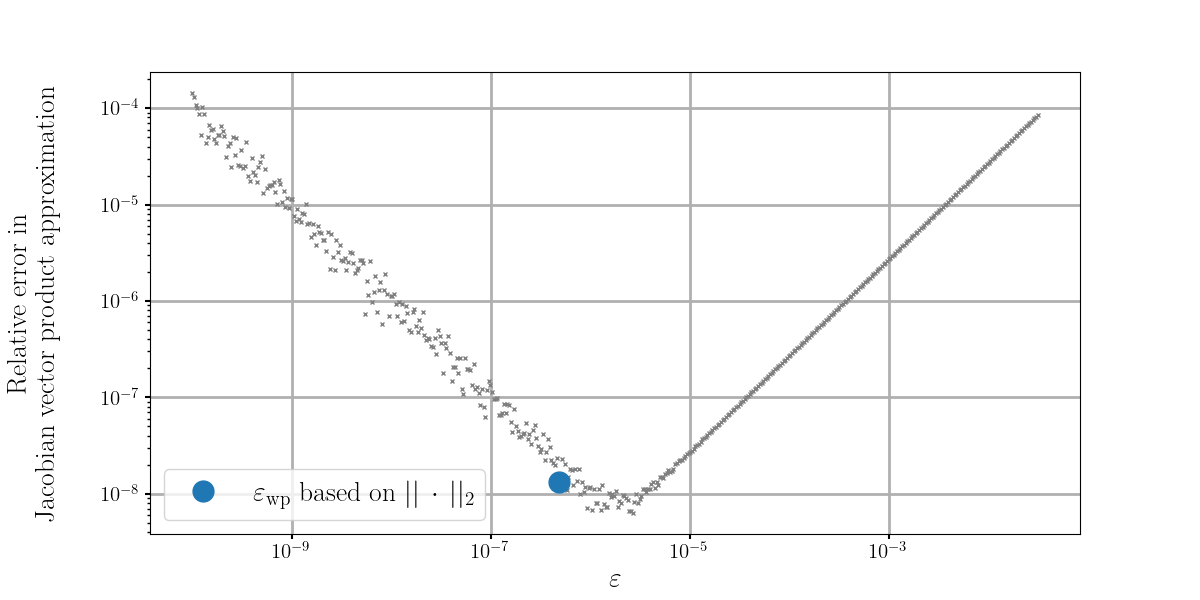
\includegraphics[width=\textwidth]{figures/epsilon_Burgers_10.png}
        \caption{
          Error in the Jacobian matrix vector product approximation as a function of $\varepsilon$, and in particular for the most popular choice $\varepsilon_\textrm{wp}$.
          The function is the right-hand side of equation (\ref{eq:ode}) from a Finite Volume method using an exact Riemann solver for Burgers' equation, over a 10 cell 1D regular mesh.
        }
        \label{fig:epsilon_burgers_10}
      \end{figure}

      \paragraph{}
      The experiment result can be seen on figure \ref{fig:epsilon_burgers_10}.
      The relative error in the approximation is shown as a function of $\varepsilon$ with small gray crosses.
      On the right part of the figure, the error decreases linearly with regard to $\varepsilon$.
      This correspond to a truncation error dominated region.
      On the left part, the error increases as $\varepsilon$ decreases.
      This correspond to a roundoff error dominated region.
      Also, this increase is not smooth as the linear decrease, because roundoff errors tend to produce more chaotic results.
      The choice of $\varepsilon$ from \cite{PerniceWalker1998} is also shown in the figure, as the large blue dot.
      As we can see, it falls into a low error region, not too much on the left, not too much on the right.

      \paragraph{}
      The issue we noticed is the following.
      Some references in the literature do not specify the norm used in equation (\ref{eq:epsilon_wp}).
      As it is most of the time the Euclidian norm $\norm[2]{\,\cdot\,}$, or 2-norm, we can assume that it is also the case when it is not specified.
      However, this means that in our example the value of $\varepsilon_\textrm{wp}$ will depend on the vector size.
      With our example, if we increase the number of cells in our mesh the typical size of the vector components stay roughly the same, so the shape of the error as a function of $\varepsilon$ should not change much from the one in figure \ref{fig:epsilon_burgers_10}.
      But if the vector components size stay the same, the 2-norm does increases with the vector dimension.
      We can even see that when the dimension is $N \gg 1$, $\varepsilon_\textrm{wp} \sim N^{-1/4}$.
      Having $\varepsilon$ to depend on $N$ did not make sense to us, as we are working with possibly large vectors in our industrial applications.
      That is why we decided to use a variation from what is currently found in the literature: we will use the norm $\norm[2]{\,\cdot\,} / \sqrt{N}$ that can be seen as a scaled 2-norm.
      We then get a new strategy for the choice of $\varepsilon$ that we note $\varepsilon_{\textrm{wp}, N}$.

      \begin{figure}
        \centering
        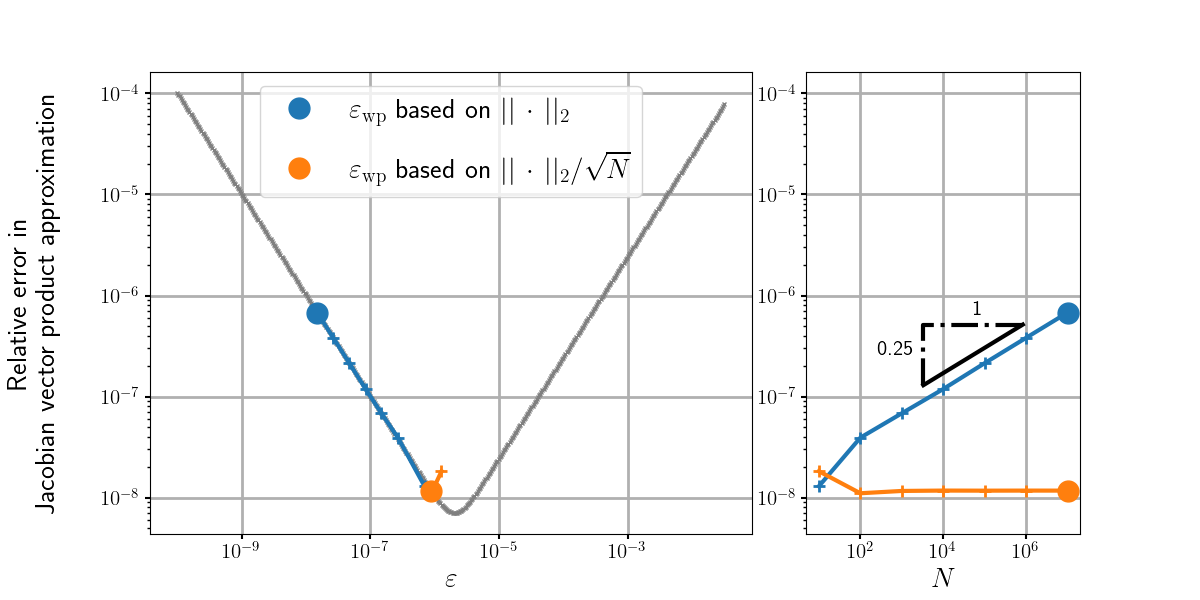
\includegraphics[width=\textwidth]{figures/epsilon_Burgers.png}
        \caption{
          Error in the Jacobian matrix vector product approximation as a function of $\varepsilon$ (left) and of the dimension $N$ (right).
          On the left figure, colored cross markers correspond to the values computed on a mesh of $10^1$, $10^2$, ... cells, and circle markers to the last value with $10^7$ cells.
          Grey cross markers on the left figure correspond to a mesh of $10^7$ cells.
        }
        \label{fig:epsilon_burgers}
      \end{figure}

      \paragraph{}
      We compared the two strategies on the same test case, while increasing the number of cells from 10 to 100, 1000, ..., up to $10^7$.
      Figure \ref{fig:epsilon_burgers} shows the result of this experiment.
      On the left, we see that the shape of the relative error as a function of $\varepsilon$ when $N = 10^7$ is similar to when $N = 10$, albeit the roundoff error dominated region is more regular.
      In particular, the ideal trade off between the two error types did not move a lot.
      We see that as expected, the value or $\varepsilon_\textrm{wp}$ decreases: this translate as the fact that the blue dot moved to the left.
      When looking at the error as a function of the dimension $N$, we can even recover the $-1/4$ expected slope.
      In the right figure we see in fact a $1/4$ slope but the error is inversely proportional to the value of $\varepsilon$ so if the error \PS{varies in} $N^{1/4}$, then $\varepsilon_\textrm{wp}$ \PS{varies in} $N^{-1/4}$.
      Because of the shape of the error as a function of $\varepsilon$, if $\varepsilon_\textrm{wp}$ changes with $N$ it will eventually end up increasing the error.
      This is an undesired feature.
      Our new choice $\varepsilon_{\textrm{wp}, N}$ on the other hand does not change a lot when $N$ increases.
      Therefore, the error level stays the same no matter the dimension.

      \paragraph{}
      The same numerical experiment was made on a more complex case: the 1D Euler equations.
      Here, the function $f$ corresponds to the right-hand side of equation (\ref{eq:ode}) given by a centered Finite Volume method used as the spatial discretisation method, in which the interface flux are defined as an average of left and right fluxes.
      This means the Riemann solver just averages the left and right fluxes.
      This spatial method is known for its instability when used in an actual solver, but it is useful in this experiment as the analytic Jacobian matrix is easy to derive, contrary to methods using more complex Riemann solvers.
      This physical model assigns 3 degrees of freedom in each cell.
      We will use the primitive variables.
      The vector $x$ corresponds to a uniform density of $1\si{\kilogram\per\cubic\meter}$, a velocity equal to a sine making one period over the mesh and of amplitude $10\si{\meter\per\second}$, and uniform pressure of $10^5\si{\pascal}$.
      The vector $v$ is a random vector in $\left[0, 1\right]$ as before, where the first component is scaled by $10^{-3}$, the second by $10^{-2}$, and the third by $10^{2}$, in order to impose $10^{-3}$ relative perturbations.

      \begin{figure}
        \centering
        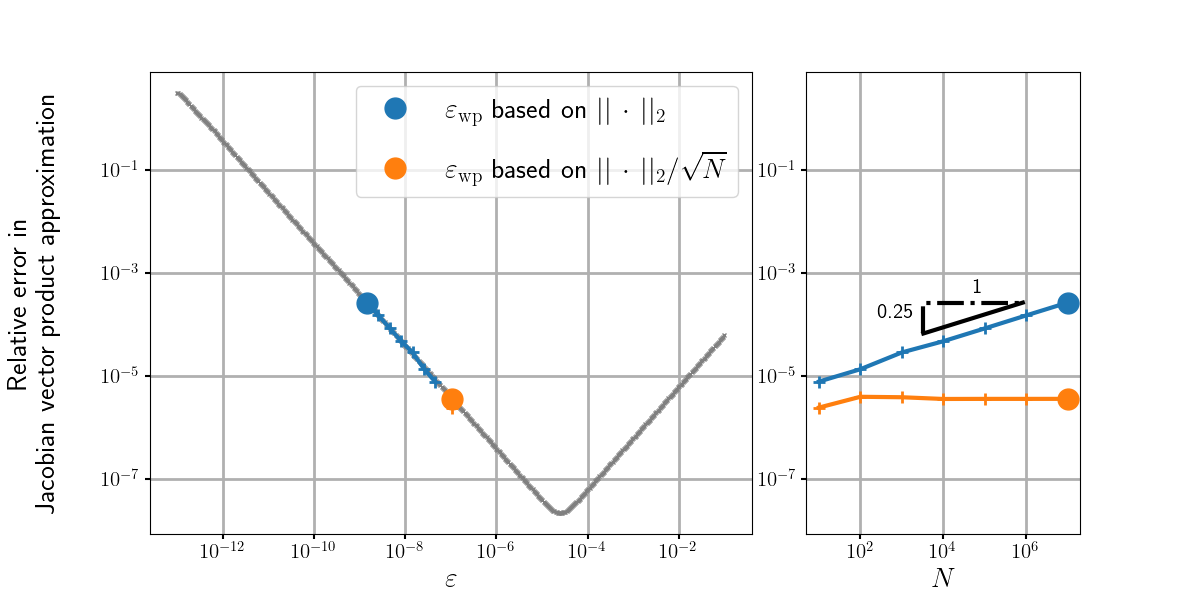
\includegraphics[width=\textwidth]{figures/epsilon_Euler.png}
        \caption{
          Error in the Jacobian matrix vector product approximation as a function on $\varepsilon$ (left) and of the dimension $N$ (right).
          The function is the right-hand side of equation (\ref{eq:ode}) from a Finite Volume method using a centered scheme for the Euler equations over a regular 1D mesh.
          On the left figure, colored cross markers correspond to the values computed on a mesh of $10^1$, $10^2$, ... cells, and circle markers to the last value with $10^7$ cells.
          Grey cross markers on the left figure correspond to a mesh of $10^7$ cells.
        }
        \label{fig:epsilon_euler}
      \end{figure}

      \paragraph{}
      Figure \ref{fig:epsilon_euler} shows the corresponding results.
      As for the previous experiment, $\varepsilon_\textrm{wp}$ depends on the dimension $N$, and then the associated error ends up increasing as $N$ grows.
      Our correction $\varepsilon_{\textrm{wp}, N}$ does not exhibit the same drawback.
      Even if it does not fall at the bottom of the error curve, it at least does not lead to a larger error.

      \paragraph{}
      In this late case, we see that at the beginning the two errors were close.
      In the first one, their starting position were a bit different.
      This is largely due to the randomness of this analysis: the one used to construct the $x$ and $v$ vectors.
      In fact, it would be unwise to draw conclusion from the position of the points in figures \ref{fig:epsilon_burgers} and \ref{fig:epsilon_euler}.
      Changing the choice of vectors, or the function $f$, or even the randomness in the vectors is enough to modify their position.
      For example, we can not conclude anything from the fact that $\varepsilon_\textrm{wp}$ is almost at the bottom of the error curve in figure \ref{fig:epsilon_burgers}.
      It may as well be a bit mort en the side.
      What we can use from this analysis, however, is the tendencies that choices of $\varepsilon$ show.
      The main conclusion is then that with our strategy we removed a dependency of the relative error on the dimension, which makes sense as this dependency is not expected a priori.

      \paragraph{}
      The issue of this analysis is that it relies on extremely simple examples.
      The function $f$ in our actual applications is in fact much more complicated than the two we used here.
      But in order to do this analysis we need to be able to compute the relative error, and this means we need to be able to compute a Jacobian matrix vector product analytically.
      Unfortunately this is not possible for our applications.
      If it was, we would not even need to introduce the approximation (\ref{eq:matrix_free}) and therefore to do this analysis.


  \chapter{Analyse de la méthode JFNK dans CEDRE}
    \section{Comparaison entre la matrice jacobienne explicite et la formulation sans matrice}
      \subsection{Sphère hypersonique}
      \subsection{Profil RAE dans un écoulement transsonique turbulent}
    \section{Utilisation de la formulation sans matrice sur un nouveau modèle de fluide}
      \subsection{Modèle Multi-températures}
      \subsection{Sphère hypersonique}
        \subsubsection{Modèle réactif complet}
        \subsubsection{Modèle réactif simplifié}


\part{Intégration temporelle à grand pas de temps}

  \chapter{Analyse d’une nouvelle catégorie d’intégrateurs temporels}

  \chapter{Analyse d’une nouvelle catégorie d’intégrateurs temporels}
    \section{Présentation de \emph{Jaguar}}
    \section{Analyse}
      \subsection{Analyse de l'ordre : convection d'un tourbillon isentropique}
      \subsection{Analyse de la robustesse : tourbillon de Taylor--Green}
      \subsection{Analyse de la rapidité : LS89}



\pagebreak
\bibliography{bibliography.bib}
\bibliographystyle{ieeetr}
\addcontentsline{toc}{chapter}{Bibliographie}

\end{document}
